\section{Performance Evaluation} \label{sec:exp}
We present a comprehensive experimental study to validate the performance and theoretical underpinnings of our proposed methods. We begin by outlining the experimental setup.

\subsection{EXPERIMENT SETTINGS}

\noindent \textbf{Algorithms.} Against a set of strong, adapted baselines, we evaluate three versions of our newly proposed strategies, including:

\noindent $\bullet$ \textbf{\dualtree},  dual-index framework without fine-grained pruning;

\noindent $\bullet$ \textbf{\dualtreeopt}, \dualtree enhanced with our cost-aware pruning, using the optimal dimensionality derived from the \textbf{rigorous theoretical model} based on \textbf{Mix Normal Distribution};

\noindent $\bullet$ \textbf{\dualtreefast}, \dualtree enhanced with pruning, using the dimensionality derived from the \textbf{fast, simplified model} based on the approximation that the proportion of variance is of linear relation with the distance precision.

Leading methods for partially-dynamic kNN joins, while not purpose-built for the fully-dynamic regime, can be adapted to provide one-sided acceleration for fully-dynamic workload. To demonstrate the global advantage of our dual-sided architecture, we benchmark against these methods as baselines, including: 1). Scan: A brute-force approach that recomputes the join after each update, serving as the performance floor; 2). idistance \cite{jagadish2005idistance}: A representative strong method for high-dimen\-sional partially dynamic kNN join where only the query set is updated; (3). Spheretree \cite{yang2014continuous}: A representative method for partially dynamic kNN join where only the reference set is updated; (4). \hdrtree \cite{ukey2022efficient}: An ablation baseline using only an \hdrtree on $U$, where forward kNN searches require a linear scan of $I$; (5). \deltatree \cite{cui2003contorting}: An ablation baseline using only a \deltatree on $I$, where RkNN searches need full scans on $U$.

Given our focus on high-stakes, low-tolerance applications, we exclusively evaluate exact kNN join methods and do not compare against approximate algorithms.

\noindent \textbf{Datasets and Hardware.} 
%
Our experiments are conducted on 8 real-world datasets, summarized in Table~\ref{tab:dataset}. These datasets span a wide range of dimensionalities (128 to 4096) and application types. All experiments were run on a machine equipped with dual Intel(R) Xeon(R) Gold 6342 CPUs, 500GB of RAM,and running Ubuntu 22.04.1LTS.
\begin{table}[htb]
\centering
\caption{Dataset Summary}
\label{tab:dataset}
\begin{tabular}{|c|c|c|c|}
\hline
\textbf{Dataset} & \textbf{No. of Records} & \textbf{No. of Dims} & \textbf{Type}\\
\hline
    NUS-WIDE & 260,000 & 128 & Image\\
    Fashion-MNIST & 60,000 & 784 & Image\\
    Audio & 53,000 & 192 & Audio\\
    Cifar & 50,000 & 512 & Image\\
    Trevi & 100,000 & 4096 & Image\\
    Sun & 79,000 & 512 & Image\\
    Enron & 95,000 & 1369 & Text\\
    Millionsong & 1,000,000 & 420 & Audio\\
\hline
\end{tabular}
\end{table}

\noindent \textbf{Evaluation Protocol.}
 Our evaluation is structured in three parts to validate our core contributions: (a)~\textbf{Core Performance Analysis:} Among the applied datasets, we conduct an in-depth parameter sensitivity study for the \textbf{mixed workload} and evaluate the influence of the update process of the \dualtree index on the classic high-dimensional dataset \textbf{NUS-WIDE} which is widely-adopted \cite{hussain2024gradual}. We supplement this with comparison on \textbf{single update types} to analyze the performance of the new methods and baselines on specific workload types. (b)~\textbf{Generality and Robustness:} We evaluate all methods on the seven additional datasets  to demonstrate the general applicability of our approaches. (c)~\textbf{Validation of the Cost Model:} We empirically verify our theoretical model's accuracy for all 8 datasets. And for representative datasets, we plot the trend of the processing time for the leaf nodes of the \dualtree with the variance of the pruning dimensionality.

\subsection{EXPERIMENT EVALUATION}
\noindent\textbf{CORE PERFORMANCE ANALYSIS}. Our core performance evaluation, conducted on the NUS-WIDE dataset, centers on a detailed parameter sensitivity study for the mixed workload. To provide attribution for the performance observed under this mixed load, we supplement the analysis comparisons on each of the three single update types. 

\noindent \textit{\textbf{Parameter sensitive study.}} We conduct an parameter sensitivity study on NUS-WIDE under a mixed workload, the most representative fully-dynamic scenario. The mixed workload is a stream of three update types: insertions into the query set (\(U\)), insertions into the reference set (\(I\)), and deletions from \(I\). Deletions from \(U\) are omitted because they are trivial and need no kNN or RkNN search.
\begin{comment}
The total dataset (NUS-WIDE) is randomly split into a \textbf{query pool} (50\%) and a \textbf{reference pool} (50\%). In each test, we vary exactly one of three parameters—the initial size of \(U\) and \(I\), the total number of updates, or the number k of neighbors required. Across all experiments, we keep the initial sizes of \(U\) and \(I\) equal and match the numbers of insertions and deletions to simulate a balanced update stream. And each inserted and deleted data point is sampled uniformly at random.
\end{comment}
\noindent(1). \textit{Varying Update Workload.} In figure \ref{fig:sub-a}, the performance of four of the baseline methods (Spheretree, \hdrtree, Scan, and idistance) is tightly clustered and orders of magnitude slower than other approaches. For clarity, we consolidate their results into a single band representing their performance range. This convention is used throughout our experiments to denote groups of similarly performing baselines that are significantly outperformed by our framework. Unsurprisingly, the total time cost for all methods increases with the number of updates, as each update requires a corresponding set of kNN or RkNN operations. Within our proposed methods, the fine-grained pruning provides substantial gains: \dualtreefast is approximately 28.4\% to 35.6\% faster than the foundational \dualtree, and \dualtreeopt further improves upon this by another 8.7\% to 9.1\%. Crucially, our dual-index architecture demonstrates a clear advantage over single-index approaches. \dualtree outperforms the strongest single-index baseline, \deltatree, by up to 26\%. This is because \dualtree's \hdrtree component efficiently localizes the impact of updates on $I$ via RkNN search, an operation that forces \deltatree into a costly brute-force scan of $U$. This benefit far outweighs the minor overhead of maintaining the \hdrtree structure. The \hdrtree baseline performs even worse, as the computational cost of the mixed workload is more heavily influenced by forward kNN searches---a task for which the \deltatree is specialized. Other baselines, such as Spheretree and idistance, exhibit even poorer performance as they lack both bidirectional acceleration and an effective, targeted dimensionality reduction strategy. Notably, even under a high update rate where the number of updates equals the initial set size, our proposed methods---particularly \textbf{\dualtreeopt} and \textbf{\dualtreefast}---maintain a significant and stable performance advantage over all baselines, demonstrating their robustness to substantial dataset evolution.

\begin{comment}
In this experiment, time cost for all 8 methods consistently increase with the update number. This is because larger number represents more times of kNN search for the inserted queries into $U$ and more times of RkNN search for the inserted reference points into $I$ to locate their affected queries in $U$ and more times of kNN search for the affected queries to repair their kNN lists. \dualtreeopt, which is the fastest method, is approximately 8.7\% to 9.1\% faster than \dualtreefast, which is the second fastest method.
And \dualtreefast shows a substantial advantage over \dualtree, being faster by approximately 28.4\% to 35.6\%. The time cost of \deltatree is at most 1.26 times that of \dualtree. This is because \dualtree demonstrates superior performance over \deltatree when dealing with data insertion into $I$ and deletion from $I$, because it conducts more efficient RkNN search to locate the affected queries in $U$ based on its \hdrtree component while \deltatree only has an index structure on $I$, thus performing brute RkNN search. These significant advantages effectively outweigh the additional overheads incurred by \dualtree compared with \deltatree for updating the structure of its \hdrtree component. As shown by the experimental results, the single \deltatree baseline consistently outperforms the \hdrtree-only baseline. This is because in a fully-dynamic mixed workload, the forward kNN search---required for both query insertions and repairs after reference deletions---constitutes the dominant computational cost, a task for which the \deltatree is specialized. Other baselines, such as Spheretree and idistance, exhibit even poorer performance as they lack both the bidirectional acceleration capability and an effective, targeted dimensionality reduction strategy.
Notably, even under a high update rate of 100\% (where the number of updates equals the initial set size), our proposed methods, particularly \dualtreeopt and \dualtreefast with their fine-grained, cost-aware pruning, maintain a significant and stable performance advantage over all baselines. This demonstrates the strong robustness of our framework to substantial dataset evolution.
\end{comment}

\noindent(2). \textit{Varying Initial Set Size.} As is shown in figure \ref{fig:sub-b}, unsurprisingly, the computation times for all methods increase with the initial set size, as larger sets naturally expand the search space for both kNN and RkNN operations. Within our proposed methods, the fine-grained pruning provides substantial gains: \dualtreefast is approximately 29.2\% to 38.9\% faster than the foundational \dualtree, and \dualtreeopt further improves upon this by another 8.8\% to 9.0\%. Crucially, our dual-index architecture demonstrates a clear advantage over single-index approaches. \dualtree outperforms the strongest single-index baseline, \deltatree, by up to 23\%. 




\noindent(3). \textit{Varying the Number of Neighbors (k).} As is shown in figure \ref{fig:sub-c} The computation time for all 8 methods increases with the value k, as larger k leads to larger pruning bounds for both kNN search and RkNN search operations. Within our proposed methods, our fine-grained pruning delivers substantial performance gains. The simplified model, \dualtreefast, is 28.2\% to 36.9\% faster than the foundational \dualtree, and the rigorous model in \dualtreeopt provides a further 9.2\% to 9.7\% improvement. Crucially, the dual-index architecture itself provides a clear advantage, with \dualtree outperforming the strongest single-index baseline, \deltatree, by up to 21\%. 

\begin{figure}[t!]
    \centering
    % --- 第一行: 左上和右上两个子图 ---
    \begin{subfigure}[b]{0.48\linewidth}
        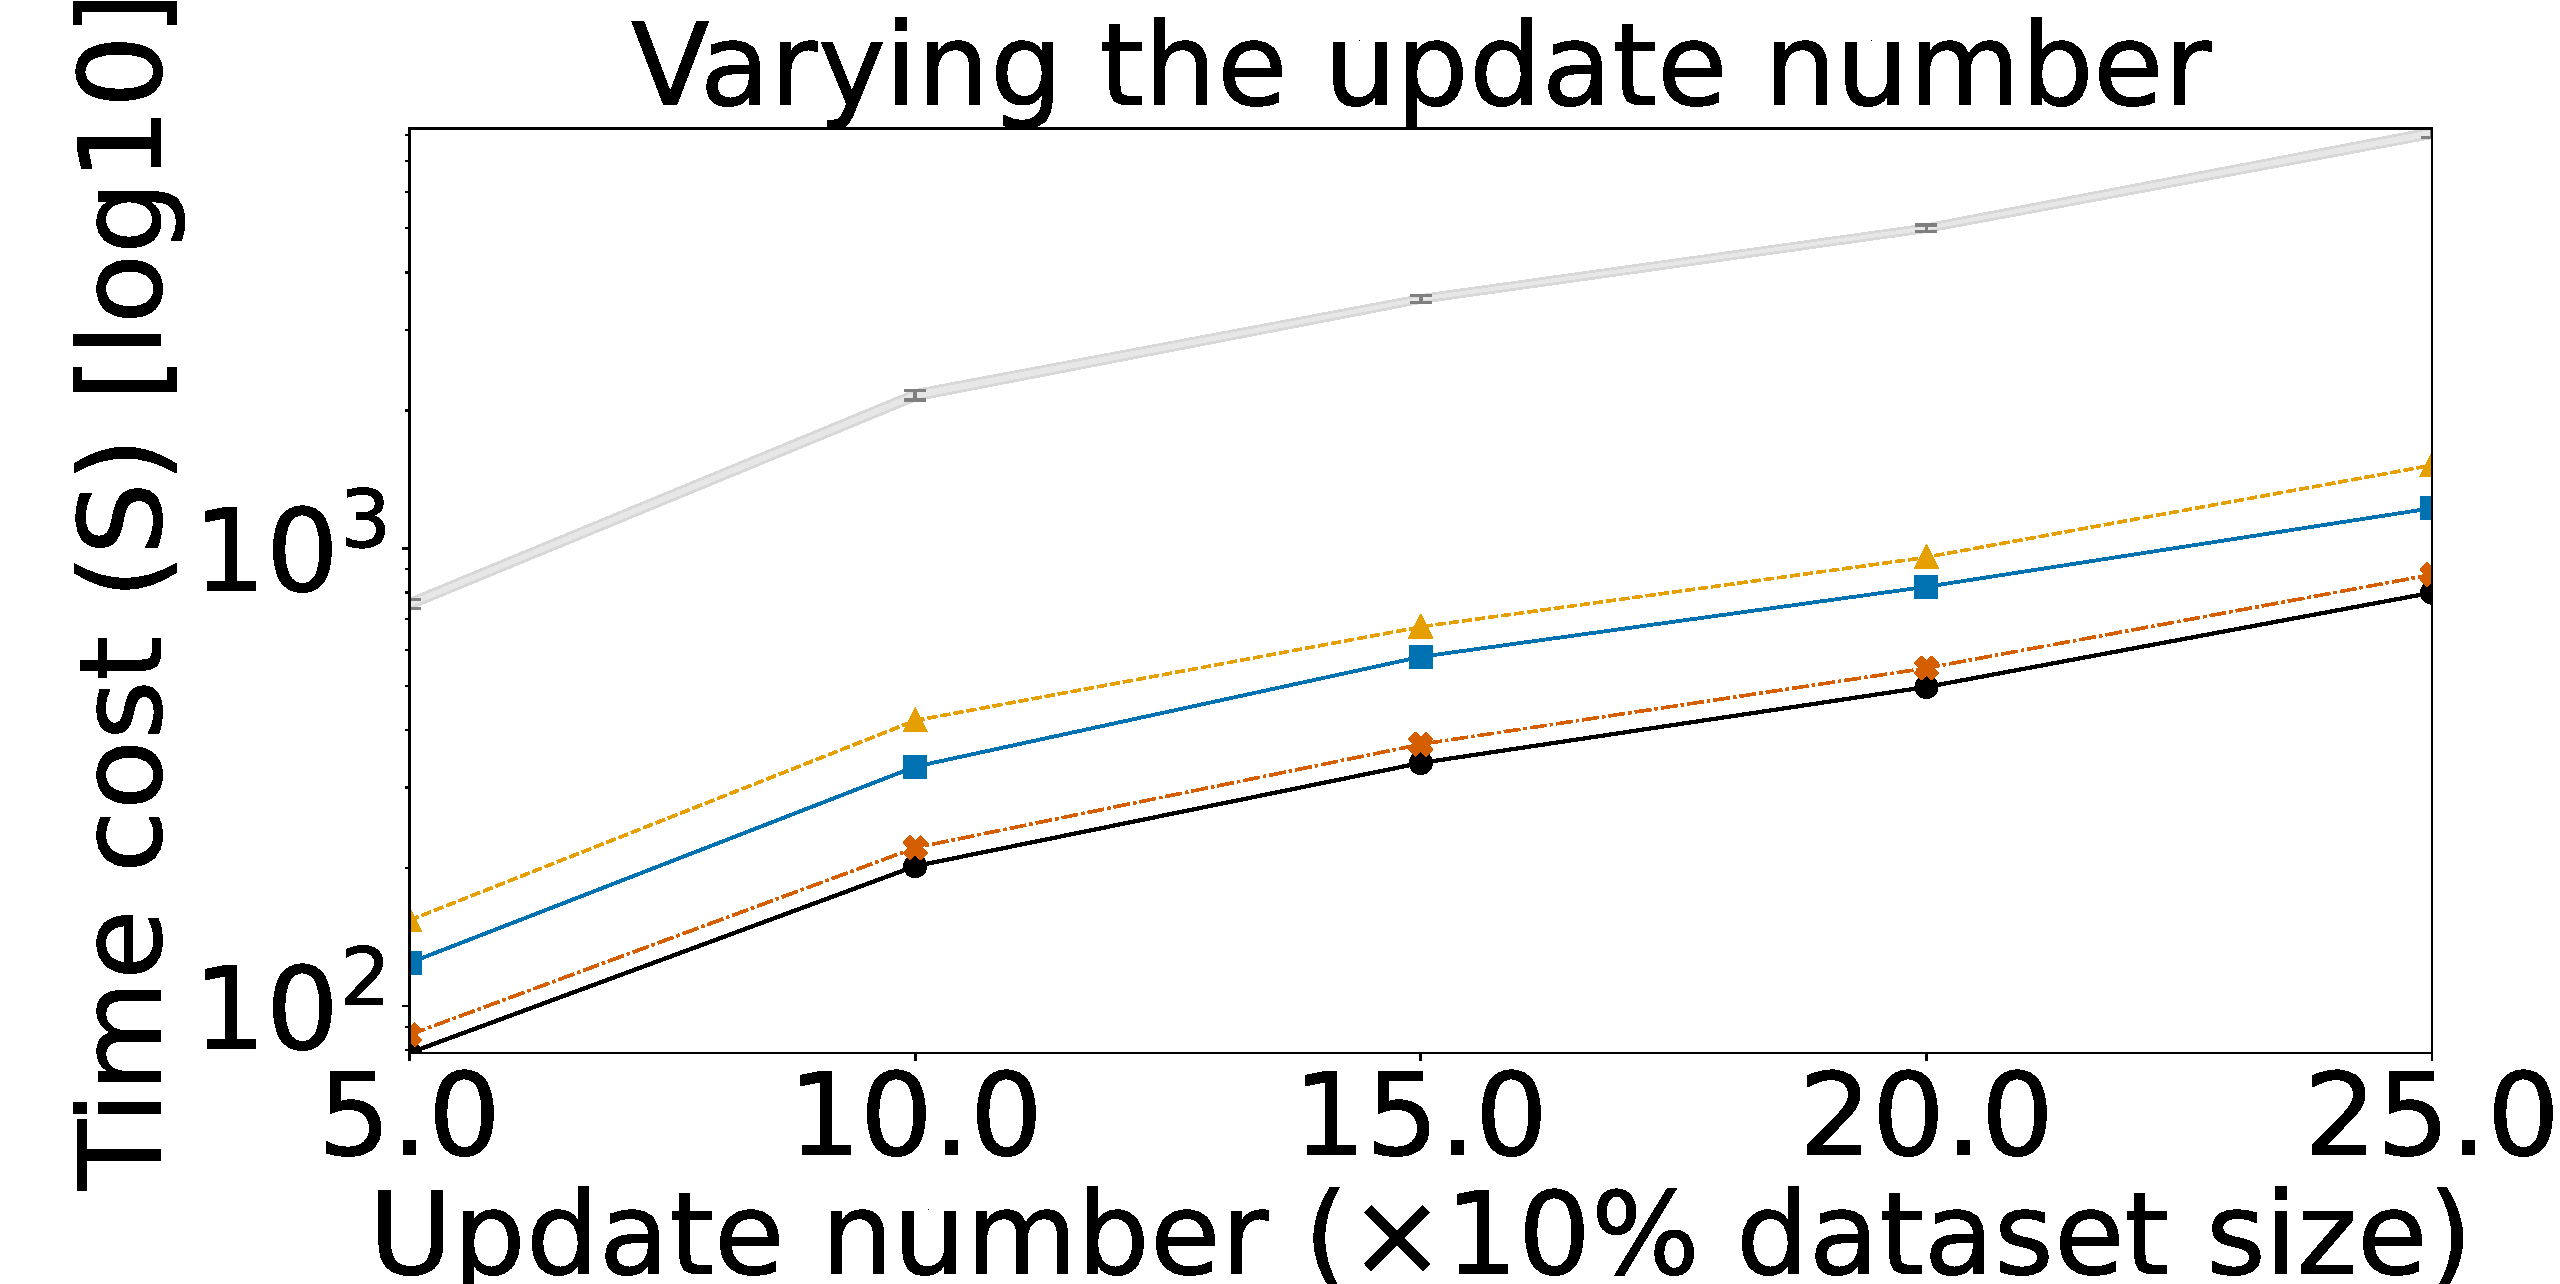
\includegraphics[width=\linewidth]{Images/realgraph/Varying the update number.pdf}
        \caption{Time cost VS update number}
        \label{fig:sub-a}
    \end{subfigure}
    \hfill % 在两张图之间创建弹性空白
    \begin{subfigure}[b]{0.48\linewidth}
        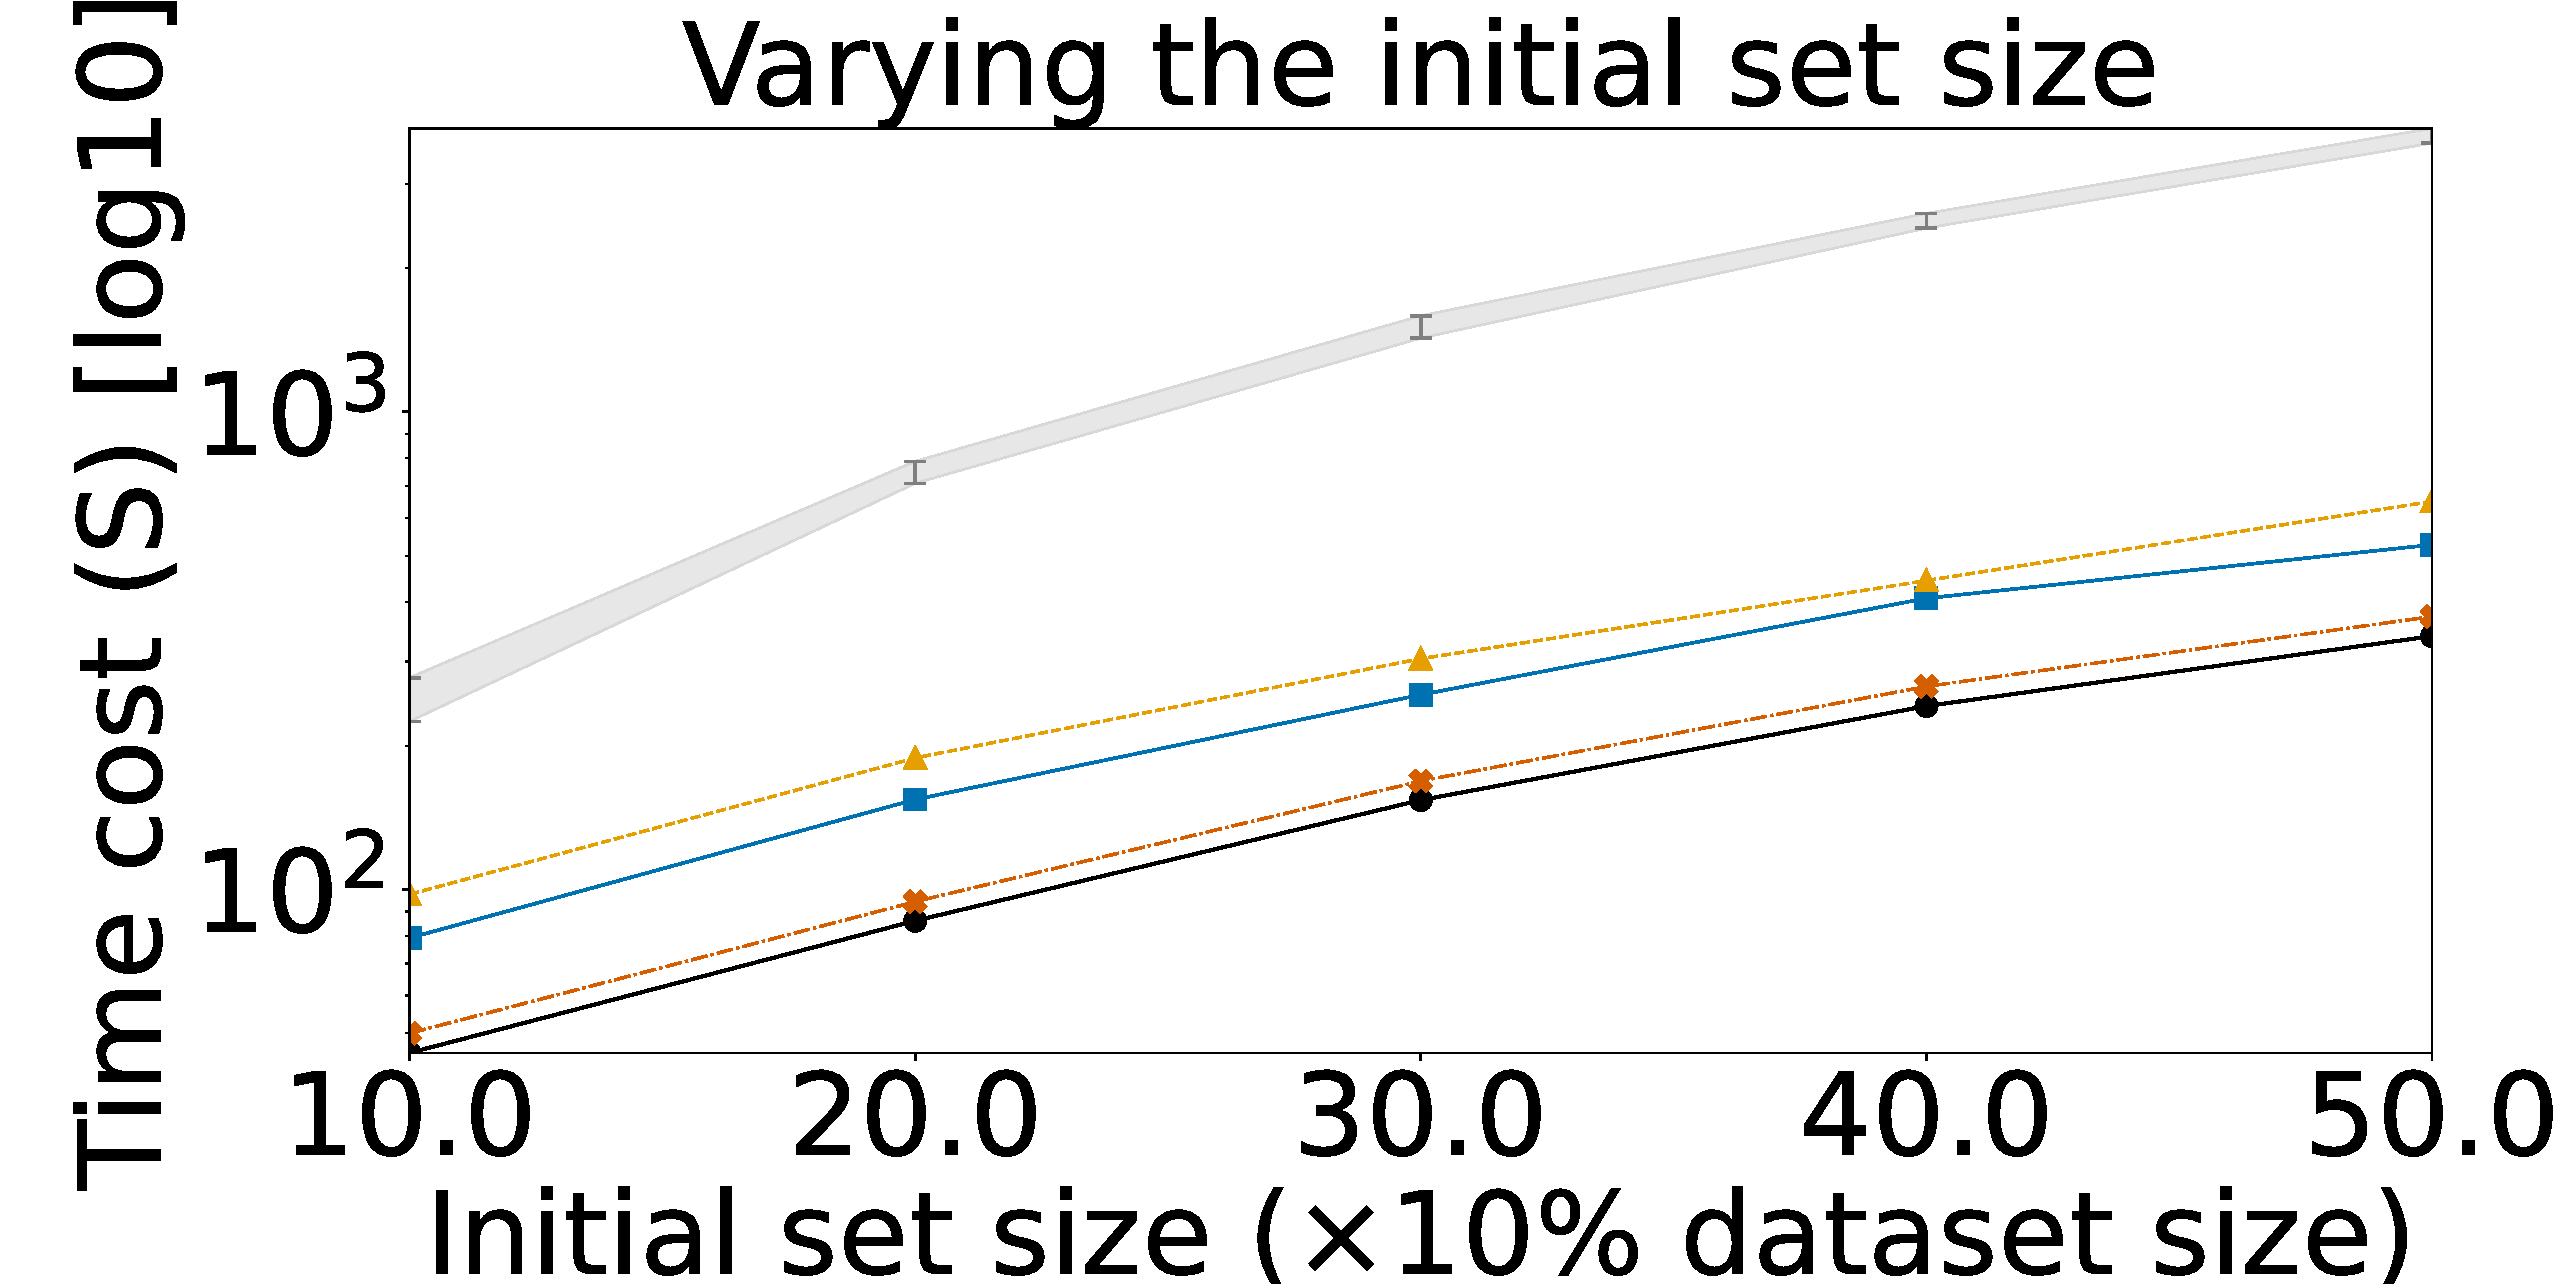
\includegraphics[width=\linewidth]{Images/realgraph/vary_initial_set_size_real_pdf.pdf}
        \caption{Time cost VS Initial set size}
        \label{fig:sub-b}
    \end{subfigure}

    \vspace{1em} % 在两行之间增加一点垂直间距 (可选，可根据排版效果调整或移除)

    % --- 第二行: 左下和右下两个子图 ---
    \begin{subfigure}[b]{0.48\linewidth}
        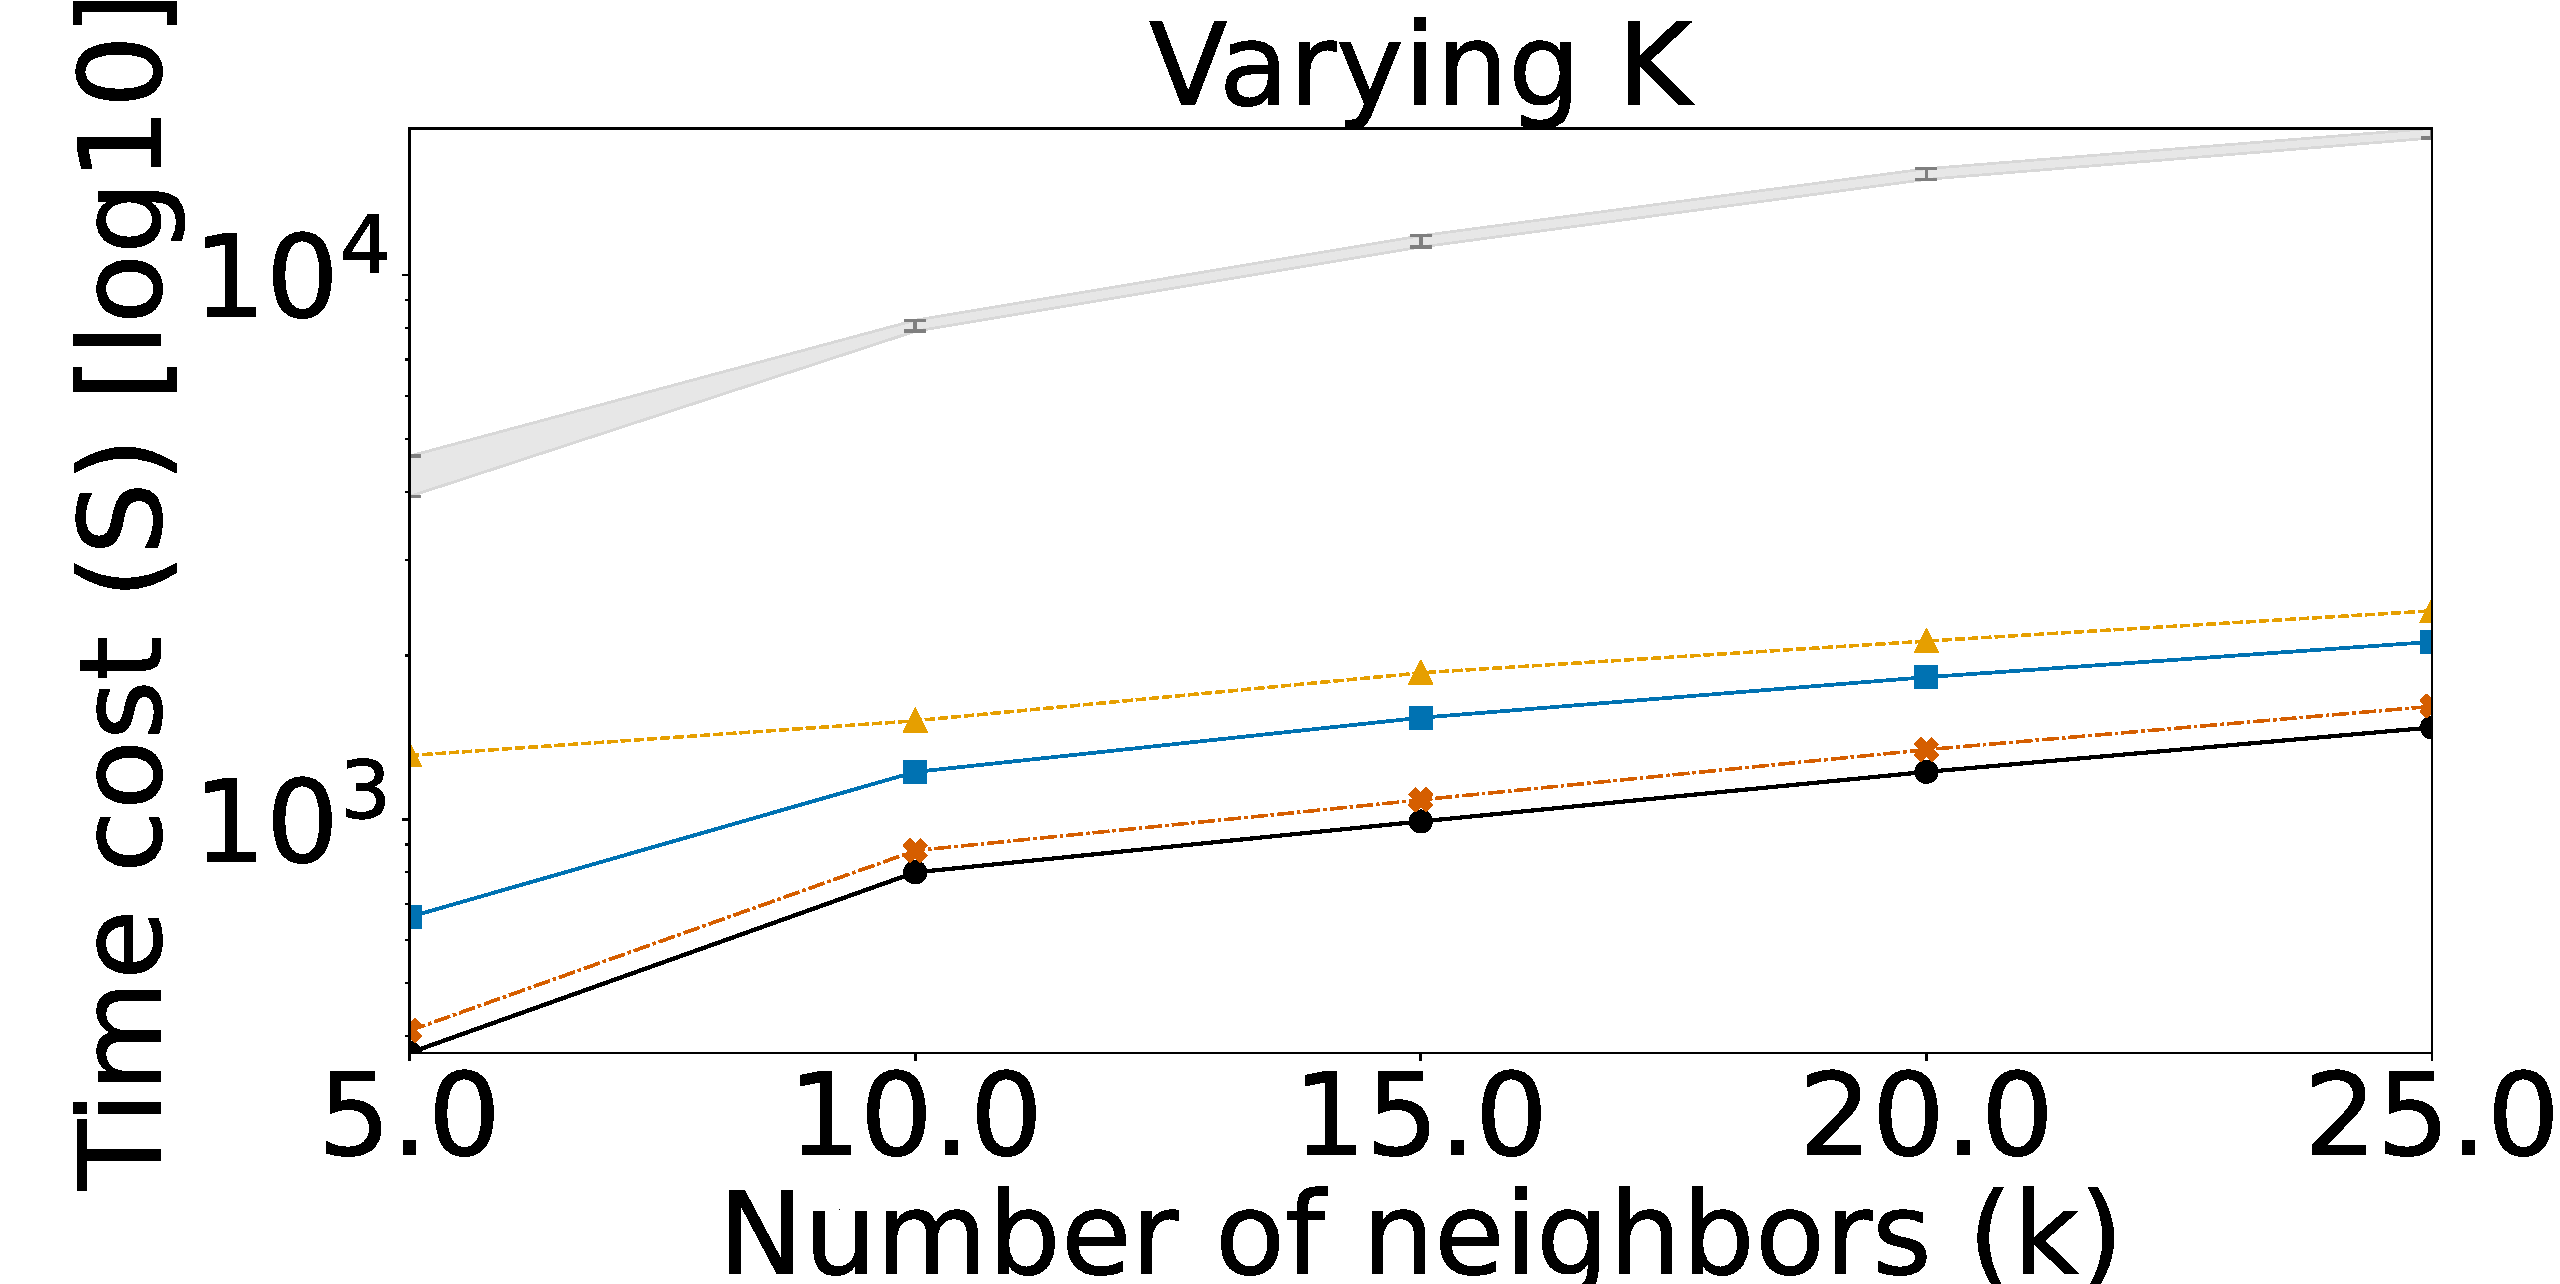
\includegraphics[width=\linewidth]{Images/realgraph/vary_k_real_pdf.pdf}
        \caption{Time cost VS Number of neighbors}
        \label{fig:sub-c}
    \end{subfigure}
    \hfill % 弹性空白
    \begin{subfigure}[b]{0.48\linewidth}
        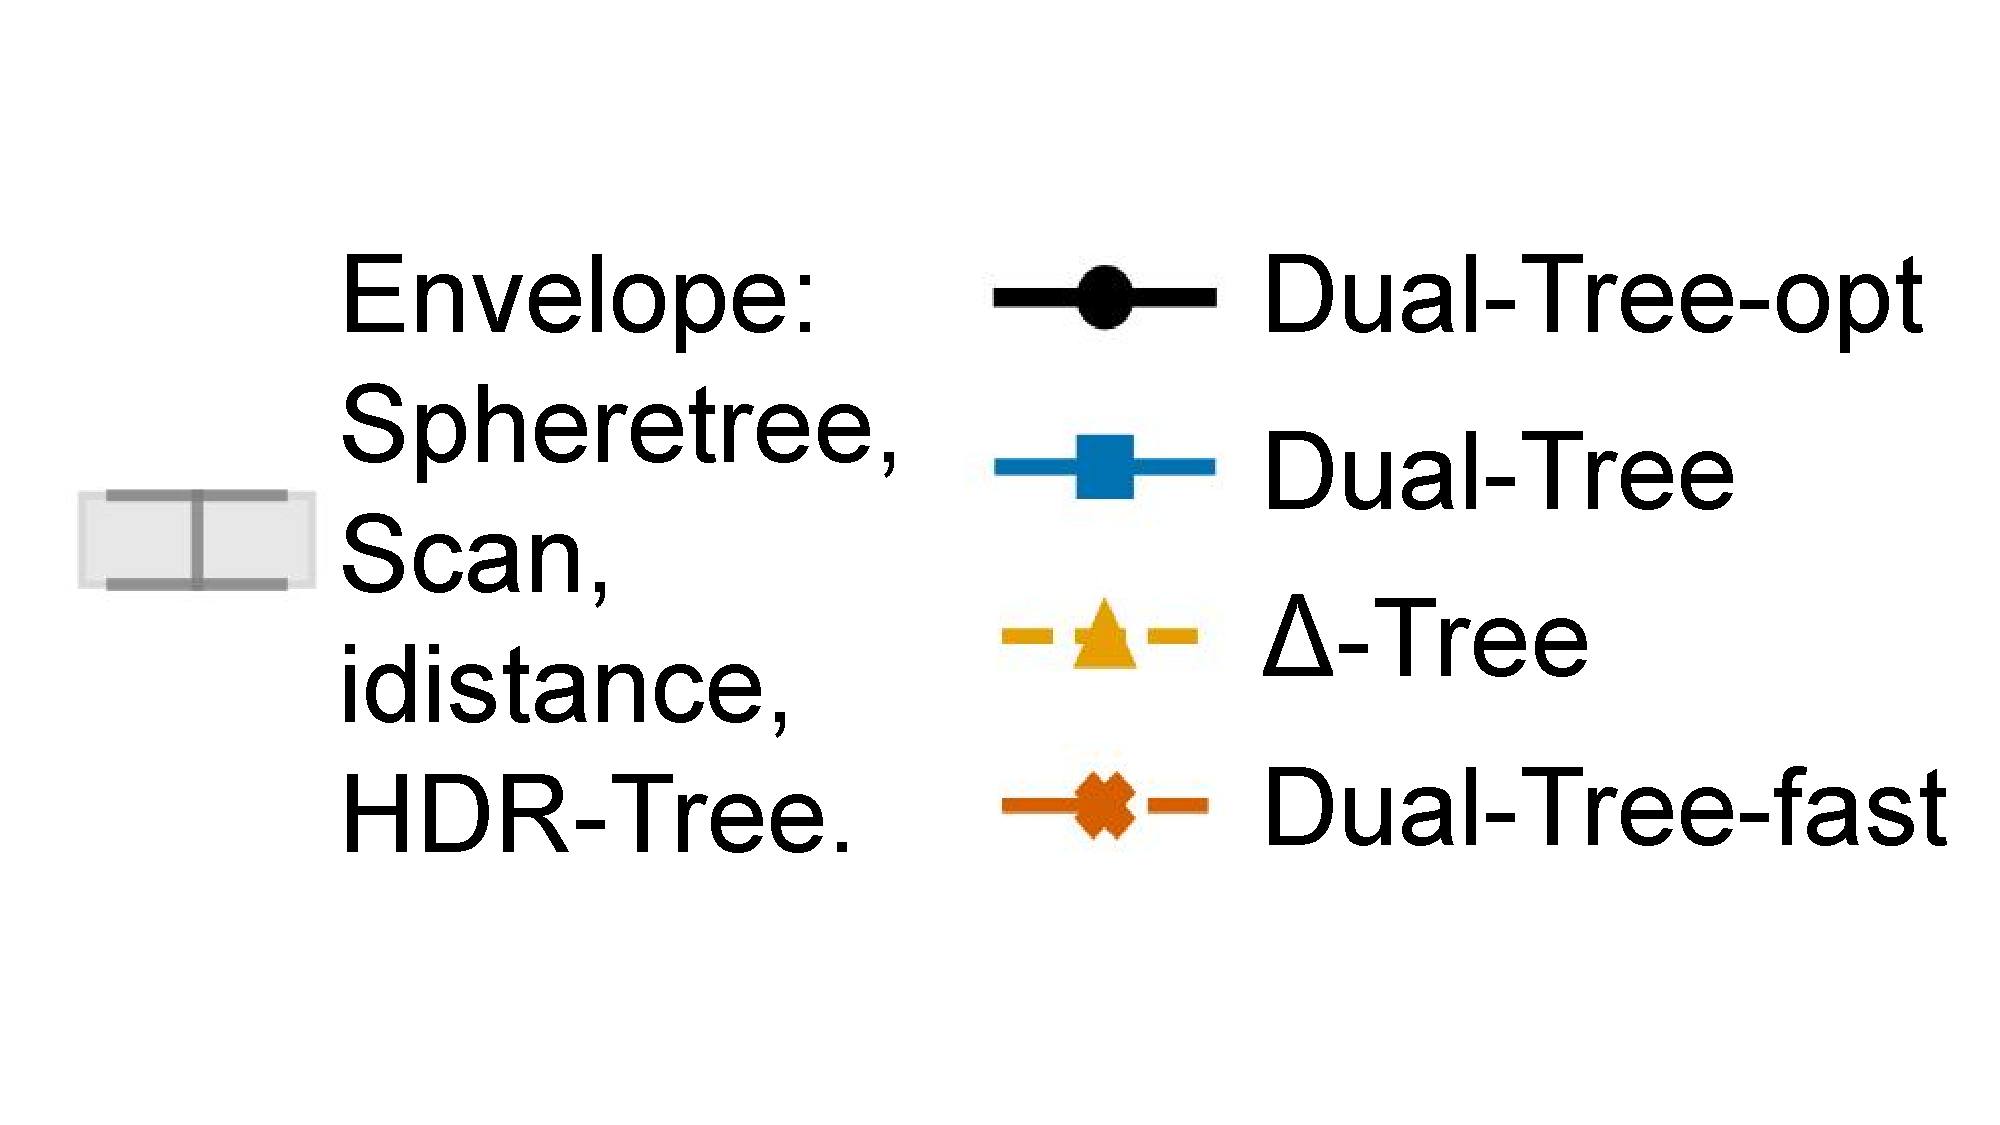
\includegraphics[width=\linewidth]{Images/realgraph/legende.pdf_2}
        \caption{Legends}
        \label{fig:subd}
    \end{subfigure}
    
    \caption{Influence of Parameters on Time Cost}
    \label{fig:main-figure-4-plots}
\end{figure}
\noindent \textbf{\textit{Performance evaluation in single update type.}} To provide attribution for the performance observed in the mixed workload, we also evaluate all methods on the three single update types under a fixed configuration, with results summarized in Table~\ref{tab:single-update-performance}. The data shows that \texttt{Delete Reference} is the most expensive workload, as it requires both an RkNN search and subsequent kNN repairs. This scenario highlights the power of our dual-index architecture: \dualtree is over 8.2$\times$ faster than \hdrtree and 1.2$\times$ faster than \deltatree on this combined workload, as it is the only framework that efficiently executes both primitives.

The results also expose the critical weakness of one-sided baselines. When a single-index method confronts an update type it was not designed for (e.g., \hdrtree handling an insertion of query), its performance degenerates to that of a linear scan, compounded by its own index maintenance overhead. In contrast, the effectiveness of our fine-grained pruning is evident. \dualtreeopt is so efficient that it outperforms the specialized single-index baselines even on their "home turf"---it is 1.9$\times$ faster than \deltatree on insertion of query and 1.3$\times$ faster than \hdrtree on insertion of reference. Finally, the data validates our choice of index components, with \deltatree and \hdrtree showing superior performance over iDistance and Spheretree, respectively, confirming they are the ideal foundation for our \dualtree framework.

\begin{table}[t!]
\centering
\caption{Performance comparison (in seconds) on single update types on the NUS-WIDE dataset. The size of the non-updated set is fixed at $S/2$, where $S$ denotes the total dataset size.}
\label{tab:single-update-performance}
\begin{tabular}{@{}lrrr@{}}
\toprule
\textbf{Method} & \textbf{$U$ ins: $\frac{S}{4}+\frac{S}{4}$} & \textbf{$I$ ins: $\frac{S}{4}+\frac{S}{4}$} & \textbf{$I$ del: $\frac{S}{2}-\frac{S}{4}$} \\
\midrule
\dualtreeopt    & 49   & 263  & 498   \\
\dualtreefast   & 54   & 275  & 545 \\
\dualtree       & 96   & 370  & 785   \\
\midrule % 在我们提出的方法和基线之间添加一个分隔线
\deltatree      & 95   & 500  & 952   \\
\hdrtree        & 884  & 360  & 6469  \\
idistance       & 798  & 507  & 7127  \\
Spheretree      & 890  & 406  & 7300  \\
Linear Scan     & 881  & 497  & 7355  \\
\bottomrule
\end{tabular}
\end{table}

\noindent \textbf{GENERALITY ACROSS DATASETS}
To demonstrate that the performance advantages of our framework are not confined to a single dataset, we evaluate all methods on seven additional real-world datasets. This tests the generality of our approach across a wide range of data distributions and characteristics. For this study, we use the mixed workload with a representative parameter configuration that the initial set size and the update number are both 25\% of the total dataset size, while k is fixed to 10.
% --- 确保您的文档导言区 (Preamble) 包含 booktabs 宏包 ---
% \usepackage{booktabs}
% (acmart 模板通常已自带)

\begin{table}[t!]
\centering
\caption{Performance (in seconds) on the mixed workload across seven additional datasets. Best performance in each column is in \textbf{bold}.}
\label{tab:generality-results}
{%
\setlength{\tabcolsep}{4pt} % 减小列间距 (默认是6pt)
\small % 在表格范围内使用小一号的字体
\begin{tabular}{@{}lrrrrrrr@{}}
\toprule
\textbf{Method} & Cifar & Audio & Msong & Sun & Trevi & Minist & Enron \\
\midrule
\dualtreeopt    & \textbf{500} & \textbf{100} & \textbf{3373} & \textbf{626} & \textbf{3716} & \textbf{244} & \textbf{3687} \\
\dualtreefast   & 524 & 115 & 3453 & 672 & 4076 & 268 & 3799 \\
\dualtree       & 700 & 170 & 5159 & 945 & 6944 & 371 & 4786 \\
\midrule
\deltatree      & 785 & 181 & 5606 & 1123 & 9851 & 545 & 5387 \\
\hdrtree        & 900 & 358 & 15288 & 2475 & 19482 & 1612 & 7473 \\
idistance       & 862 & 275 & 14155 & 1883 & 17326 & 1120 & 6338 \\
Spheretree      & 912 & 367 & 15997 & 2485 & 21166 & 1694 & 7959 \\
Linear Scan     & 978 & 378 & 16044 & 2422 & 22866 & 1789 & 8255 \\
\bottomrule
\end{tabular}%
}
\end{table}

The results, summarized in Table~\ref{tab:generality-results}, confirm that the superiority of our proposed methods is consistent across all tested datasets. \dualtreeopt achieves the best performance in every case.

The data clearly demonstrates the advantage of the dual-index architecture itself. Our foundational \dualtree framework consistently outperforms the strongest single-index baseline, \deltatree, achieving speedups ranging from 1.06$\times$ (on Audio) to 1.47$\times$ (on Minist). This validates that our symmetric design effectively handles the bidirectional nature of the fully-dynamic workload.

Building upon this architectural advantage, our fine-grained pruning delivers substantial additional gains. Compared to the strongest baseline (\deltatree), \dualtreeopt achieves an average speedup of 1.88$\times$ across all seven datasets. The performance gap is most pronounced on the high-dimensional Trevi dataset, where \dualtreeopt is 2.65$\times$ faster. The other baselines, whose performance is often clustered together and significantly slower, are consistently outperformed by a wide margin. These results affirm the robustness and general applicability of our \dualtree framework and the cost-aware pruning model.

\noindent \textbf{VALIDATION OF COST MODEL.} We now empirically validate the accuracy of our cost-aware dimensionality selection model. The validation is twofold: a qualitative analysis to visually confirm the cost-dimensionality trade-off, and a quantitative analysis to measure the precision of our model's predictions.

\noindent\textbf{\textit{Qualitative Validation.}} We first visualize the cost-dimensionality curve on the highest-dimension dataset, Trevi (4096-D), which presents the greatest challenge. We measure the execution time for the leaf nodes for both a kNN-dominant workload (query insertion) and an RkNN-dominant workload (reference insertion), varying the pruning dimensionality $d$ across a wide range. The results are plotted in Figure~\ref{fig:main-figure-two-plots}.

\begin{figure}[t!]
    \centering
    % --- 第一个子图 (左侧) ---
    \begin{subfigure}[b]{0.48\linewidth}
        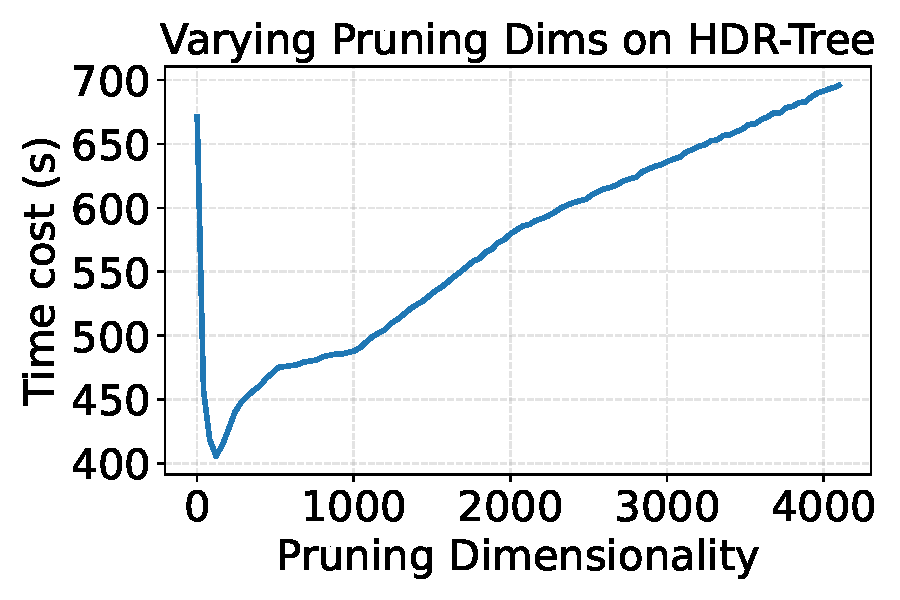
\includegraphics[width=\linewidth]{Images/realgraph/dim_hdr_pdf.pdf}
        \caption{Dims vs. Time Cost (RkNN)}
        \label{fig:sub-a_1}
    \end{subfigure}
    \hfill % 在两张图之间创建弹性空白，将它们均匀推开
    % --- 第二个子图 (右侧) ---
    \begin{subfigure}[b]{0.48\linewidth}
        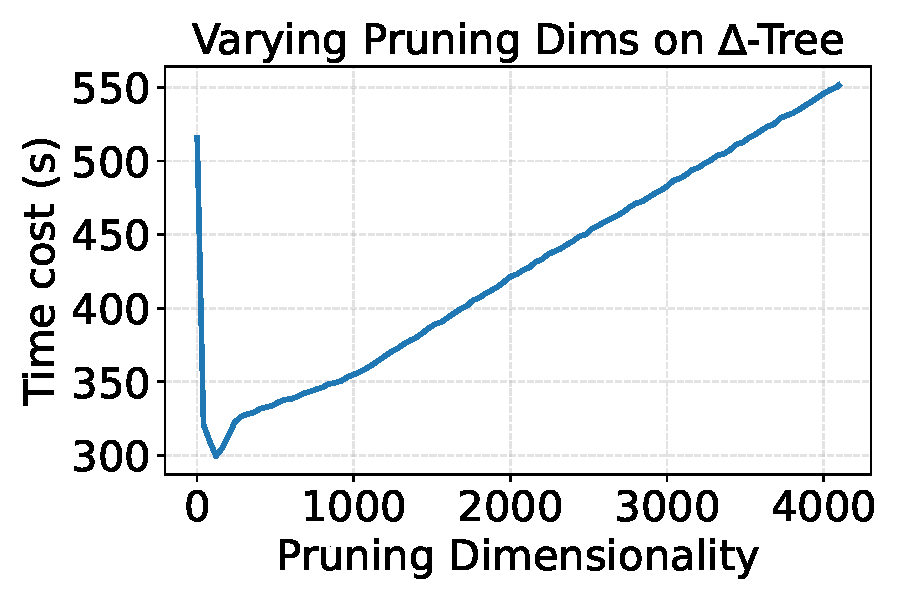
\includegraphics[width=\linewidth]{Images/realgraph/dim_delta_pdf.pdf}
        \caption{Dims vs. Time Cost (kNN)}
        \label{fig:sub-b_1}
    \end{subfigure}
    
    \caption{Cost-dimensionality curve dominant workloads.}
    \label{fig:main-figure-two-plots}
\end{figure}

As observed in Figure~\ref{fig:main-figure-two-plots}, the cost curve exhibits a distinct U-shape for both RkNN search on the \hdrtree and kNN search on the \deltatree, confirming our theoretical premise. This trend is explained by the properties of PCA. Initially, at low dimensionalities, each added dimension provides substantial pruning gains because the leading principal components capture a large fraction of the data's variance; the benefit from improved pruning accuracy far outweighs the marginal computational cost of an additional dimension. However, as dimensionality increases, the incremental information gain from later principal components diminishes. At this point, the linear increase in per-check computation cost begins to dominate, causing the total execution time to rise again.

 To quantify our model's accuracy, we conducted a validation across all 8 datasets. For both kNN-dominant (query insertion) and RkNN-dominant (reference insertion) workloads, we compare the optimal dimension predicted by our models (\dualtreeopt and \dualtreefast) against the empirically measured best dimension. The results are summarized in Table~\ref{tab:model-validation}, which reports two key metrics for both kNN and RkNN search: the relative error in the predicted dimension, and the resulting relative error in execution time. Across eight datasets (Table~\ref{tab:model-validation}), \dualtreeopt attains minimal dimensional error—including 0\% on Enron—while keeping time error below 3\%. \dualtreefast shows slightly higher dimensional error yet typically maintains time error below 5\%, providing a practical closed-form alternative with negligible performance loss. Both models effectively select a near-optimal pruning dimensionality for our fine-grained pruning stage. 
\begin{table}[t]
\caption{Validation of the cost model on eight datasets. Each cell reports \textbf{Dim/Time} error (\%).}
\label{tab:model-validation}
\centering
\begin{tabularx}{\columnwidth}{@{}l *{4}{>{\centering\arraybackslash}X}@{}}
\toprule
& \multicolumn{2}{c}{\textbf{RkNN on \hdrtree}} & \multicolumn{2}{c}{\textbf{kNN on \deltatree}} \\
\cmidrule(lr){2-3}\cmidrule(lr){4-5}
\textbf{Dataset} & \makecell{ opt \\ Dim/Time \%} & \makecell{ fast \\ Dim/Time \%} & \makecell{ opt \\ Dim/Time \%} & \makecell{ fast \\ Dim/Time \%} \\
\midrule
NUS-WIDE    & 13.9/1.1 & 14.7/1.4 & 18.5/2.3 & 23.3/2.9 \\
Cifar       & 15.3/1.8 & 18.4/2.2 & 12.8/0.4 & 15.1/0.5 \\
Sun         & 10.8/3.4 & 11.8/3.7 & 20.7/4.0 & 26.7/5.2 \\
Audio       & 25.7/2.7 & 28.8/2.5 & 25.7/0.7 & 27.7/0.6 \\
Enron       & 0.0/0.0  & 38.9/4.7 & 0.0/0.0  & 29.5/2.8 \\
MNIST       & 15.6/1.1 & 18.7/1.4 & 25.3/0.0 & 28.3/9.7 \\
Trevi       & 7.9/1.3  & 8.9/1.3  & 8.4/0.8  & 9.2/0.8  \\
Millionsong & 9.5/2.5  & 5.8/3.1  & 10.2/1.2 & 10.4/1.4 \\
\bottomrule
\end{tabularx}
\end{table}





